\documentclass[12pt,a4paper]{article}

\usepackage{float}
\usepackage{pdflscape}
\usepackage{parskip}
\usepackage[hyphens]{url}
\usepackage[hidelinks]{hyperref}
\usepackage[margin=3.5cm]{geometry}
\usepackage{graphicx}
\usepackage{subfigure}

\usepackage[bottom]{footmisc}
\usepackage{longtable}

% Stretch table cell height
\renewcommand{\arraystretch}{1.5}

%%%%%%%%%%%%%%%%%%%%%%%%%%%%%%%%%%%%%%%%%%%%%%%%%%%%%%%%%%%%%%%%%%%%%%%%%%%%%%%%
% BIBLATEX SETTINGS
%%%%%%%%%%%%%%%%%%%%%%%%%%%%%%%%%%%%%%%%%%%%%%%%%%%%%%%%%%%%%%%%%%%%%%%%%%%%%%%%
\usepackage[
backend=bibtex,
firstinits=true,    % Render first and middle names as initials
maxcitenames=2,     % Use maximum 2 names in \cite before et al.
maxbibnames=99,      % Use maximum 2 names in references before et al.
style=authoryear,
dashed=false,       % Re-print recurring author names in bibliography
]{biblatex}

% Use single quotes around titles:
\usepackage[british]{babel}
\usepackage{csquotes}

% Add a blank line between references
\setlength{\bibitemsep}{\baselineskip}

% Don't use reference months
\AtEveryBibitem{\clearfield{month}}
\AtEveryCitekey{\clearfield{month}}

% All author's names should be Last, First
\DeclareNameAlias{author}{last-first}

% Insert a comma between author and year in text citations
\renewcommand*{\nameyeardelim}{\addcomma\addspace}

% Remove 'in:' preceding article title
\renewbibmacro{in:}{}

\addbibresource{../bibliography.bib}

%%%%%%%%%%%%%%%%%%%%%%%%%%%%%%%%%%%%%%%%%%%%%%%%%%%%%%%%%%%%%%%%%%%%%%%%%%%%%%%%

\begin{document}
\begin{titlepage}
\center
\vspace*{3cm}

{\Large
    Electronics and Computer Science\\
    Faculty of Physical Sciences and Engineering\\
    University of Southampton\\[1cm]
}

Jamie Davies\\
%\href{mailto:jagd1g11@ecs.soton.ac.uk}{\nolinkurl{jagd1g11@ecs.soton.ac.uk}}\\[3cm]
\today\\[1cm]

{\large
    Enhanced Content Analysis and Information\\
    Retrieval Using Twitter Hashtags\\[1cm]
}

A project report submitted for the award of\\
MEng Computer Science\\[1cm]

\emph{Supervisor:}\\
Dr.\ Nick Gibbins\\[0.5cm]
%\href{mailto:nmg@ecs.soton.ac.uk}{\nolinkurl{nmg@ecs.soton.ac.uk}}\\[0.5cm]

\emph{Examiner:}\\
Dr.\ Klaus-Peter Zauner\\
%\href{mailto:kpz@ecs.soton.ac.uk}{\nolinkurl{kpz@ecs.soton.ac.uk}}\\


\vfill
\end{titlepage}

\section*{Abstract}
One of the key characteristics of Twitter and other microblogging platforms is the use of `hashtags' --- topical/categorical annotations provided by the authors of the posts (tweets) themselves. This flexible system was designed for the effective organisation and searching of tweets, but with Twitter facing an ever-increasing number of users and tweets it is hard for users to keep track of the vast number of hashtags in popular use. This results in data from the hashtags being fragmented and inaccurate due to the users making poor or uninformed hashtag choices.

If users are presented with a choice of relevant hashtags when writing a tweet, they are more likely to publish tweets with accurate tag data. This project aims to create an intelligent hashtag recommendation tool to improve the quality of the information we can gain from hashtags. However, whilst such a system could improve future tweets, tweets that have already been published will remain untouched by the system. Thus, the system will be extended to also retrofit hashtags to published tweets --- allowing for tweets to appear in search results for a particular hashtag even if they don't actually contain the hashtag in question.
\pagebreak

\tableofcontents

\pagebreak

\section*{Acknowledgements}
I would like to thank my supervisor, Dr.\ Nick Gibbins, for providing inspiration and guidance throughout the course of the project.

I would also like to thank Dr.\ Jonathon Hare and Dr.\ Sina Samangooei for their continued support and advice.

\section*{Statement of Originality}

The work contained within this report has not been previously submitted for a degree or diploma at any other higher education institution. To the best of my knowledge and belief, this project contains no material previously published or written by another person except where due references are made.

\pagebreak

\section{Introduction}
Collaborative tagging (sometimes referred to as social tagging) systems are designed to allow users to navigate, organise and manage online resources. The central idea behind these systems is the concept of an annotation: the action of a user applying a personalised tag to a resource. On a large scale, many of these annotations can be taken together to form a complex network of users, resources and tags --- commonly referred to as a \emph{folksonomy} \parencite{Xu:2008}.

One of the most popular applications of a folksonomy is Twitter\footnote{\url{www.twitter.com}}. `Hashtags,' which are simply any combination of letters or digits preceded by a hash character (\#), afford users the ability to create free-form tags to describe the content of their posts (tweets). Tweets can be categorized with several hashtags, thereby creating networks of tweets and users, and making it easy to find other related tweets, users and hashtags. This renders hashtags as a powerful tool in aiding the search and navigation of the billions of tweets contained within Twitter.

Despite its numerous benefits, the hashtag system presents new challenges to overcome before it can become truly useful. Due to the open nature of folksonomies, it is important that users have the freedom to create and use exactly the tags they wish to use. However, this unsupervised tagging can result in vast numbers of hashtags for users to choose from --- often including redundant or ambiguous hashtags. When posting a tweet, there is nothing stopping a user from creating an entirely new hashtag to describe something with exactly the same meaning as a collection of other hashtags. This tag redundancy can confuse users and fragment the true meaning behind the synonymous hashtags.

There is also the converse issue of tag ambiguity to consider, in which a single hashtag could be associated with many meanings and connotations. The use of these hashtags can incorrectly imply that tweets are similar and related to one another, when in fact they are from distinct unrelated categories.

Because these problems are complicating the already vast hashtag information space, an intelligent recommendation system is needed to aid users in their choice of hashtags. For example, when a user writes a tweet such as: ``\emph{The golden gate bridge looks so nice today! I LOVE SF in this weather!}'', the system should recommend hashtags such as \texttt{\#SanFrancisco}, \texttt{\#California} or even \texttt{\#sohappy}, but should not recommend hashtags such as \texttt{\#ScienceFiction}, \texttt{\#amreading} or \texttt{\#fantasy}.

Such a recommendation system would also need to aid users in the navigational and exploratory aspects of folksonomies. For example, when a user performs a search on Twitter for the hashtag \texttt{\#BGT}, the system should display not only those tweets that contain \texttt{\#BGT}, but also tweets that contain other relevant hashtags such as \texttt{\#BritainsGotTalent}, \texttt{\#VoteAttraction} or \texttt{\#VoteJackCarroll}.

\subsection{Preliminary Data Analysis}

To investigate the usage of hashtags and the problems associated with them further, a dataset of 500,000 tweets was collected from the sample Twitter stream over a time period of approximately 4.5 days. The tweets collected were filtered to ensure that they were in English, and contained at least one hashtag.

Through the use of some trivial Python scripts, it is easy to find evidence of poor hashtag choices. In particular, the most overwhelming observation is the quantity of redundant hashtags in use throughout Twitter. \autoref{tbl:redundancy} shows several hashtags taken from the dataset and their number of occurrences. Despite the tags all having exactly the same semantic meaning, the use of the tags is fragmented and spread across several tags.

\begin{table}[H]
\centering
\begin{tabular}{| l | l |}
    \hline
    \textbf{Hashtag} & \textbf{Number of Occurrences} \\
    \hline \hline
    \#peopleschoice & 94849 \\ \hline
    \#peopieschoice & 2043 \\ \hline
    \#peoplechoice  & 439 \\ \hline
    \#peoplesch     & 287 \\ \hline
    \#peopleschoi   & 269 \\ \hline
    \#peoplesc      & 230 \\ \hline
    \#peoplescho    & 219 \\ \hline
    \#peolpeschoice & 164 \\ \hline
    \#peopleschioce & 137 \\ \hline
    \#pca           & 94 \\ \hline
\end{tabular}
\caption{Occurrences of hashtags referring to the People's Choice Awards}
\label{tbl:redundancy}
\end{table}

Another interesting observation is that of the times that different hashtags are used, which varies greatly from hashtag to hashtag. Some tags are used in tweets at a fairly uniform rate (Fig.~\autoref{fig:android}), whilst others feature large spikes of usage over a short period of time (Fig.~\autoref{fig:blackfriday}). This demonstrates the communities behind the hashtags --- rather than a hashtag being used at a particular time for a particular event, some hashtags are used consistently by users to join in on a large-scale conversation.

\begin{figure}[H]
    \centering
    \subfigure[\#android]{
        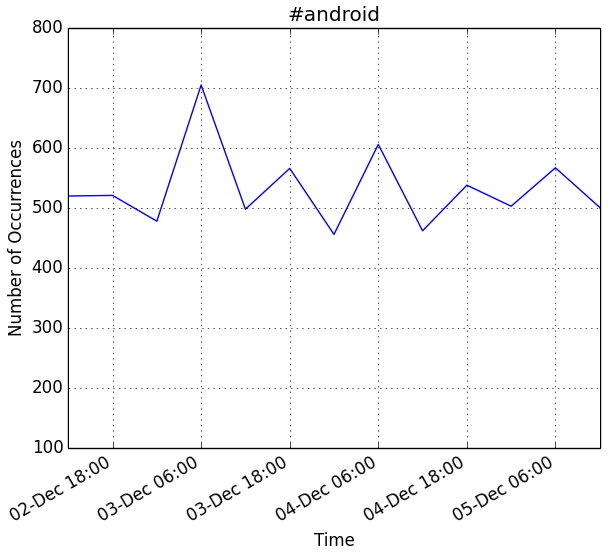
\includegraphics[width=0.75\textwidth]{android}
        \label{fig:android}
    }

    \subfigure[\#blackfriday]{
        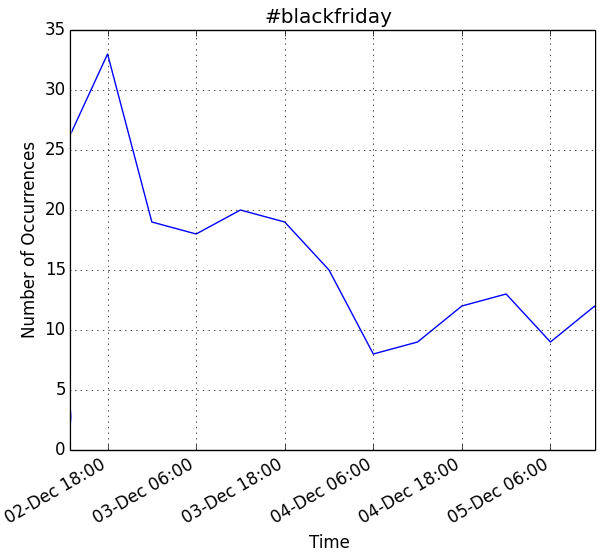
\includegraphics[width=0.75\textwidth]{blackfriday}
        \label{fig:blackfriday}
    }
    \caption{Usage of hashtags over the period that the dataset was collected.}
\end{figure}

\pagebreak

\section{Background Literature \& Related Work}
\label{sec:litreview}
The main design goals behind hashtags are to categorise tweets and allow them to show up more easily in searches\footnote{\url{https://support.twitter.com/articles/49309-using-hashtags-on-twitter}}. Whilst the task that this project is aiming to complete is novel and fairly unexplored, it is well connected with other experiments, systems and projects within the research community.

\subsection{Traditional Recommendation Systems}
Traditional recommendation systems are in place all over the web today. From music discovery services (such as Last.fm\footnote{\url{www.last.fm}}) to suggested purchases on retail sites (like on the front page of Amazon\footnote{\url{www.amazon.co.uk}}), these systems are all personalised recommendation engines that take an individual user's preferences and use them to provide suggestions tailored to that user.

Most personalised recommendation systems employ a set of techniques known as collaborative filtering. These techniques were first coined by \textcite{Goldberg:1992}, where a system named \emph{Tapestry} was created that allowed people to attach annotations to documents, and then use that information to filter the documents for other users.

One common implementation of collaborative filtering is the so-called ``user-to-user'' approach. ``User-to-user'' collaborative filtering works by taking the preferences of a user $A$, and finding a small subset of other users in the system that have similar preferences. For each user $B$ in the subset, any items that $B$ has adopted that $A$ hasn't are added to a ranked list of suggestions. $A$ is now more likely to adopt items in the list than the items of another random person \parencite{Schafer:2001}.

Another approach to provide relevant recommendations to a user is the use of content-based recommendation systems. This is a type of system that recommends items relevant to other items by comparing the details and descriptions of the items themselves. This can be extended to suggest items for a user by comparing a content-based description of the user's preferences with the descriptions of the items \parencite{Pazzani:2007}.

A key issue with content-based filtering is that the recommendations can only be as accurate as the algorithm used to derive a user's profile. There are a number of algorithms available to build user profiles, depending upon the context, but essentially a content-based profile is created using a weighted vector of item features. The weights mark the importance of each feature to the user, and can be computed from individually rated content vectors.

\textcite{Cantador:2010} studied and evaluated a number of content-based recommendation models based upon the premise of user and item profiles being described in terms of weighted lists and tags. Through their experiments they found that models that focused on user profiles outperformed the models oriented towards item profiles in nearly every test. They go on to suggest that a better way of profiling users would be through the use of tag clustering.

Instead of limiting recommendation systems to the accuracy of their classifiers, a common approach is incorporate relevance feedback techniques. Relevance feedback is a process that was originally designed for information retrieval, and works on the assumption that a user can not always correctly encapsulate into a query what it is they are searching for. It works by allowing a user to create an initial query to which an initial set of results is returned. Out of these initial results, the user can then mark certain results as relevant or irrelevant, and this information is then submitted and used to refine the original query and return more relevant results to the user \parencite{Salton:1990}.

\textcite{Utiyama:2006} showed that it is possible to combine collaborative filtering, content-based filtering and relevance feedback techniques into one system to provide better recommendations.

\subsection{Assigning Labels with Machine-Learning Techniques}
Although there exists a long history of research into traditional recommendation algorithms, the data structure of a folksonomy is distinct from those found in traditional problems. This has led to a new generation of supervised learning classification algorithms which can be applied to the problem of assigning labels to resources.

In order to facilitate the comparison of resources, tags and users, aggregate projections of the data can be constructed. This reduces the dimensionality of the data by sacrificing some information \parencite{Schmitz:2006}. There are two main classes of algorithms that perform this task: feature \emph{selection}, which reduces the size of a dataset by selecting a subset of the data, and feature \emph{extraction}, which uses the existing data to generate entirely new features. Despite the improved results that feature extraction can provide, their computational cost and memory requirements can often make them impractical for use on the extremely large datasets common with Folksonomies \parencite{Gemmell:2009}.

One compromise to this trade-off is to use an algorithm such as Hebbian Deflation, which approximates the outputs of the intensive feature extraction techniques, but with lower computational cost and memory requirements \parencite{Oja:1985}. \textcite{Gemmell:2009} used this approach coupled with a K-Nearest Neighbour classifier to find appropriate tags for a given resource. This was done by finding `neighbouring' users: ``Neighbours are selected only if they have tagged the query resource and tags are selected for the recommendation set only if they have been applied by the neighbour to the resource.'' It was tested on data from the popular bookmarking site Delicious\footnote{\url{http://delicious.com/}} and from Citeulike\footnote{\url{http://www.citeulike.com/}}, a tool that enables researchers to manage and discover scholarly references, and it was found to be a successful approach with giving results.

\textcite{Niwa:2006} took a different approach to overcome the limitations of collaborative filtering. Using a modified version of the TF-IDF \parencite{Salton:1988}, they calculate the affinity level between users and tags (where affinity level is a measure of how frequently a user uses a particular tag), and then use this to calculate the similarity between tags. These similarity measures are then clustered using a custom clustering algorithm to provide a set of recommended tags for a given user and resource. This enabled them to adjust the level at which a user's preferences were taken into account when determining recommendations, as well as providing a simple solution to the tag redundancy issue found across most Folksonomies.

Another popular machine-learning approach to the folksonomy tag recommendation problem is the use of a Naive Bayes classifier. Naive Bayes has been an accepted tool in information retrieval for a long time, with some early literature dating back over 50 years \parencite{Maron:1960}, and has recently been seeing a renaissance within the machine-learning community.

As shown by \textcite{DePessemier:2010}, Naive Bayes can be easily adapted and extended to work in the context of providing recommendations to match a query or a set of user preferences. In particular, their algorithm relied upon the general user preferences for cases where the classifier produced an uncertain outcome, and became more context specific on a sliding scale as the classifer gave more certain probabilities.

\subsection{Other Approaches to Hashtag Recommendation}
Even though providing hashtag recommendations and suggestions is still a new and largely unexplored field, there have been several efforts to improve the hashtag experience for Twitter users.

The current hashtag system on Twitter (\autoref{fig:twittersuggest}) uses a non-personalised auto-complete tool to provide suggestions to the user. Whenever a hash symbol (\#) is typed in the tweet composer, the system simply suggests hashtags starting with the letters that the user has typed so far. These suggestions are chosen from a tiny subset of hashtags, taken from a mixture of those currently trending\footnote{Trending hashtags are those with the highest rise in usage within a given time period.} and from the user's history. Whilst better than not having suggestions at all, this system is only truly useful in one of two specific use cases: when the user knows the starting letters of a trending hashtag they want to use, or are trying to recall a hashtag that they have previously used. This system does not help the user choose the correct hashtag for the content of their tweet.

\begin{figure}[htpb]
    \centering
    
\includegraphics[width=0.5\textwidth]{twittersuggest.png}
    \caption{Twitter's current hashtag suggestion system.\label{fig:twittersuggest}}
\end{figure}

By assuming that the primary purpose of hashtags is to categorise tweets and improve searching (as Twitter envisioned), \textcite{Zangerle:2011} created a system that recommends hashtags for a tweet by taking hashtags from other tweets that are textually similar to the query. The similarity between tweets is calculated with the TF-IDF model. The hashtags are then extracted from the similar tweets, ranked according to how similar the tweets were to the original query, and returned as a list of suggestions to the user. A number of different ranking algorithms were tested, but this was found to be the most successful.

After studying the advantages of providing personalised recommendations in retail situations on a per-user basis, \textcite{Kywe:2012} realised that a similar approach towards hashtags could prove fruitful. Hashtag use varies from user to user, with some users using the latest trending hashtags, other users only using a specific set or type of tag, and with some users barely using them at all. They proposed a personalised hashtag recommendation system that considers both user preferences and the query tweet content: the system creates a ranked list of hashtags from both the most similar users and most similar tweets. This gave promising results, although it was noted that this may not be the best recommendation system for all types of tweets and hashtags.

\textcite{Shepitsen:2008} used a hierarchical agglomerative clustering algorithm to profile users and provide personalised recommendations in collaborative tagging systems. They found that clusters of tags can be effectively used to ascertain a user's interests, which could then be used in a traditional content-based recommendation approach. This technique worked well, particularly for dense folksonomies such as Last.fm.

Observers of social media have realised that hashtags play a dual role within the online microblogging communities, such as Twitter. On one hand, hashtags fulfil the design goals that Twitter created them to accomplish (bookmarking and improving search); on the other hand, however, they serve as a badge of community membership: connecting users together. \textcite{Yang:2012} took this duality into account when attempting to create a hashtag recommendation system by training a SVM (support vector machine) classifier with a variety of features taken from the tweet metadata to overcome the duality and suggest relevant hashtags.

\pagebreak

\section{Requirements}
There are two main requirements the system in this project is aiming to fulfil. It must:
\begin{itemize}
    \item Allow users to compose and publish tweets whilst suggesting hashtags relevant to the content of their tweets.
    \item Allow users to search for a hashtag and view related tweets, including those that don't contain that hashtag.
\end{itemize}

\subsection{Functional Requirements}
\begin{enumerate}
    \item \label{func:publish} The system must allow the user to log in and publish tweets to their Twitter account.
    \item \label{func:suggest} The system must provide hashtag recommendations as the user is creating a tweet.
    \item \label{func:search} The system must perform a hashtag search through a large dataset of tweets and return all relevant tweets, including those that do not contain the search query.
    \item \label{func:genmodel} The system must use information from a large dataset of tweets to generate a model representing each hashtag.
    \item \label{func:compmodels} The system must be able to compare tweets against its representational hashtag models.
    \item \label{func:stream} \emph{Optional:} The system must be able to update its classification models using information from the live Twitter stream.
    \item \label{func:probabilities} \emph{Optional:} The system must provide probabilities for how likely a hashtag is to be related to a tweet.
\end{enumerate}

\subsection{Non-Functional Requirements}
\begin{enumerate}
    \item \label{nfunc:web} The system must be accessible via a web interface.
    \item \label{nfunc:easy} The system must be responsive and easy to use.
    \item \label{nfunc:qsearch} The system must be able to perform searches quickly.
    \item \label{nfunc:qsuggest} The system must be able to make hashtag recommendations quickly.
    \item \label{nfunc:graphs} The system must be able to produce visualisations to provide an easy way to interpret the hashtag recommendations/assignments.
    \item \label{nfunc:mobile} \emph{Optional:} The system must be accessible via mobile web browsers.
\end{enumerate}

\pagebreak

\section{Design}
    \subsection{Architecture}
        \subsubsection{Processing Framework}
        \subsubsection{Classifier}
    \subsection{Interface}
        \subsubsection{API Endpoints}
        \subsubsection{Web Interface}

\pagebreak

\section{Implementation}
    \subsection{Stream Processing}
    \subsection{Classification System}
        \subsubsection{Training}
        \subsubsection{Classifying}
        \subsubsection{Optimisation}
        \subsubsection{RESTful Interface}
    \subsection{Web Application}
        \subsubsection{Framework}
        \subsubsection{Authentication}
        \subsubsection{Connecting to Classifier}

\pagebreak

\section{Testing}
    \subsection{Strategy}
    \subsection{Unit Testing}
    \subsection{Classification Testing}
    \subsection{User Interface Testing}
    \subsection{Requirements Validation}

\section{Conclusion}
    \subsection{System Evaluation}
    \subsection{Project Management}
    \subsection{Future Work}

\pagebreak

\begin{landscape}
    \appendix
    \section{Time Management}
    \label{appendix:gantt}
    This is a Gantt chart showing the scheduled progression through the different aspects of the project.

    \begin{figure}[H]
        \centering
        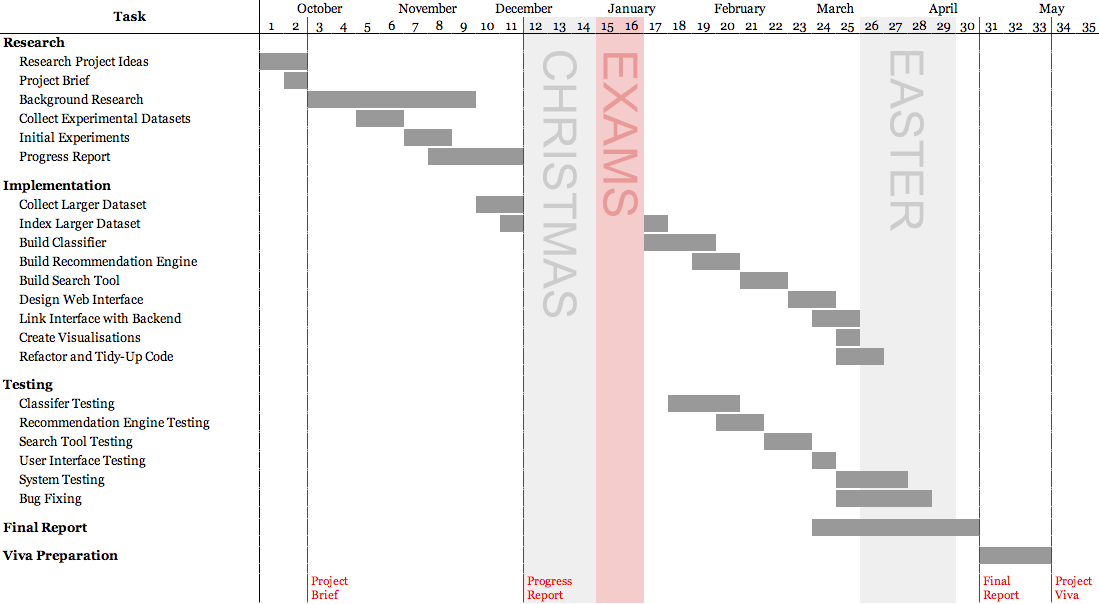
\includegraphics[height=0.85\textwidth]{gantt.png}
    \end{figure}
\end{landscape}

\section{Testing Plans \& Results}
\pagebreak

\section{REST API Interface}
\pagebreak

\section{Original Project Brief}
\vspace*{-3cm}
\hspace*{-2.4cm}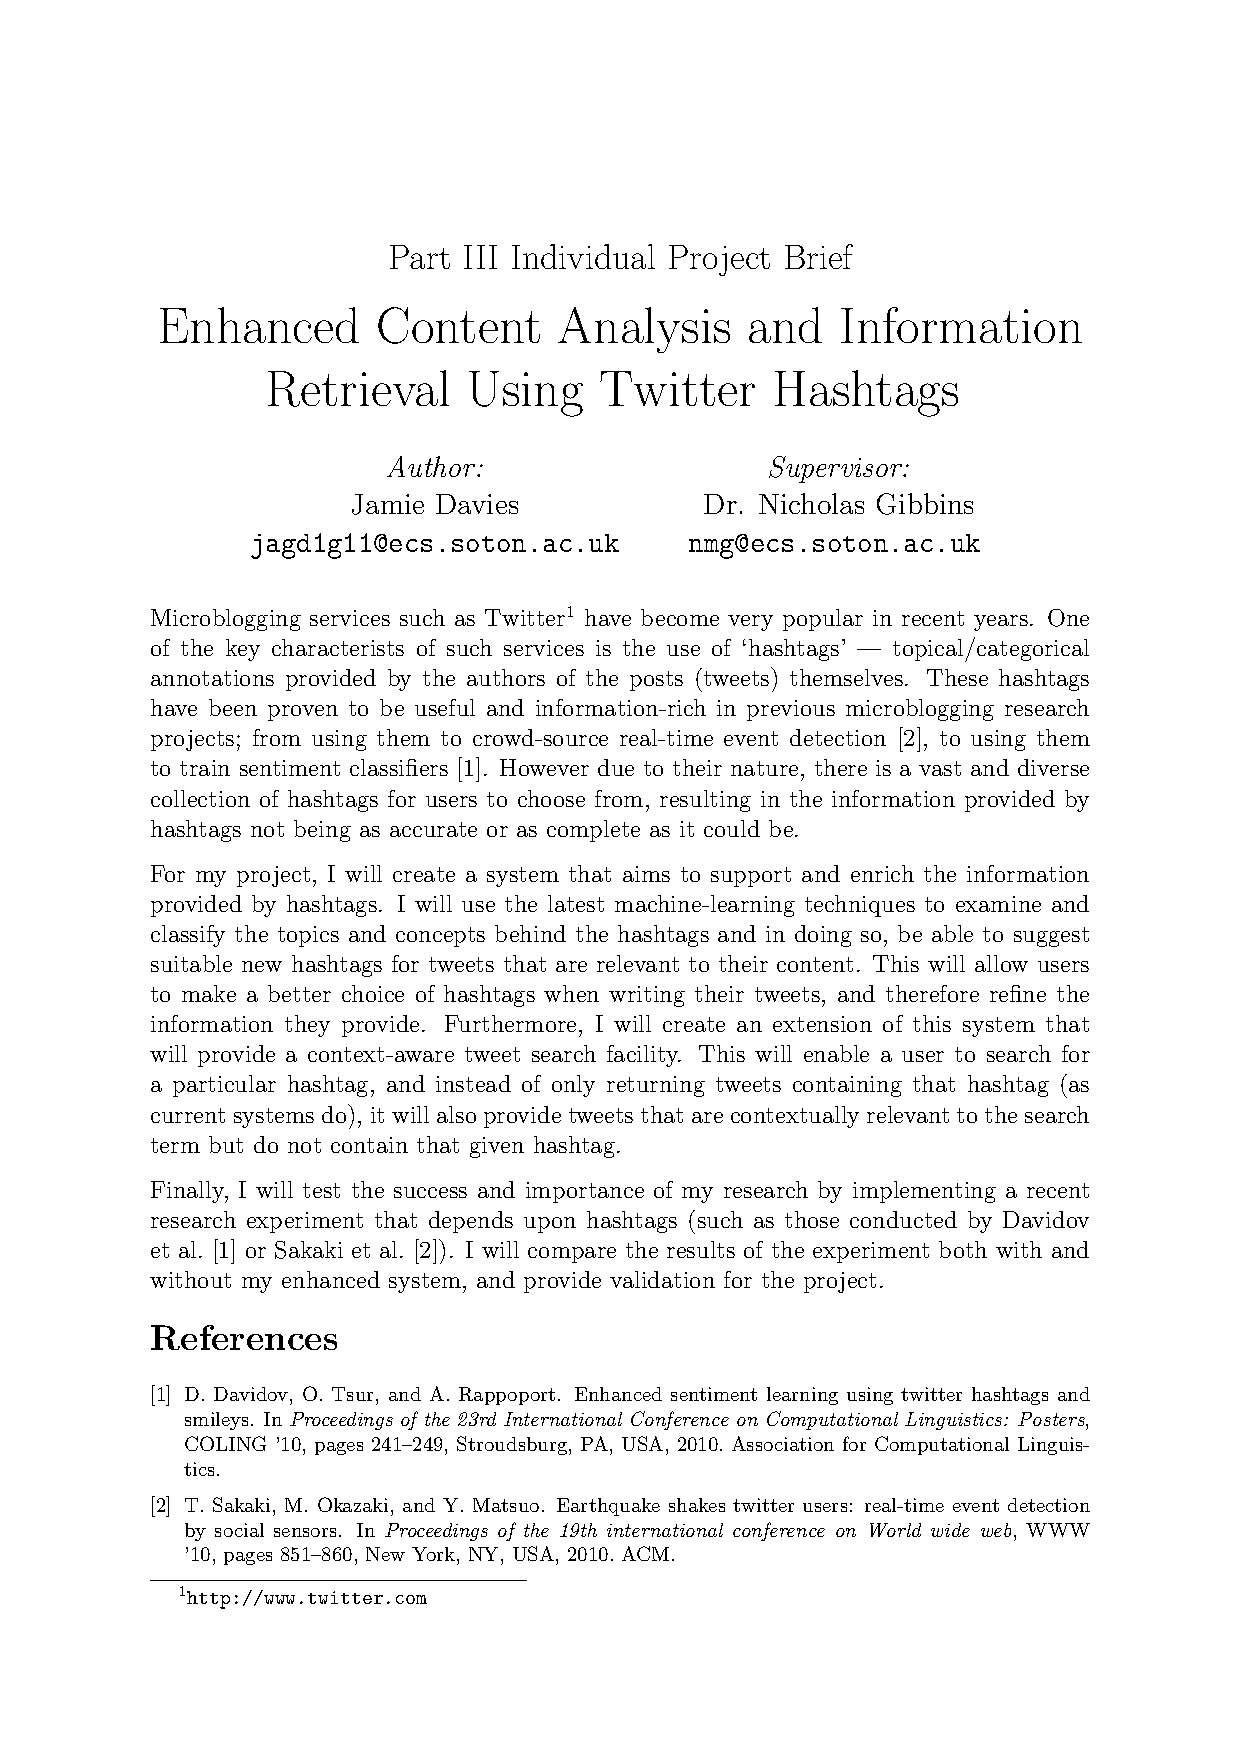
\includegraphics[scale=0.9]{../brief/brief.pdf}
\pagebreak

\setcounter{secnumdepth}{0}
\section{References}
{\footnotesize \printbibliography[heading=none]}

\end{document}
